\documentclass[review]{elsarticle}

%%% Le da el formato final -- una vez aceptado
%\documentclass[final,authoryear,5p,times]{elsarticle}
%\documentclass[final,authoryear,5p,times,twocolumn]{elsarticle}

\usepackage{lineno,hyperref}
\modulolinenumbers[5]

\usepackage{amssymb}
\usepackage{multirow}
\usepackage{subfig}
\usepackage{amsmath}
\usepackage{algorithm} 
\usepackage{algpseudocode} 
\usepackage{hyperref}
\usepackage{makecell}
\usepackage{amsmath}
\usepackage{relsize}

\usepackage{tikz}
\usetikzlibrary{matrix,decorations.pathreplacing,calc,fit}


\journal{Astronomy and Computing}

%%%%%%%%%%%%%%%%%%%%%%%
%% Elsevier bibliography styles
%%%%%%%%%%%%%%%%%%%%%%%
%% To change the style, put a % in front of the second line of the current style and
%% remove the % from the second line of the style you would like to use.
%%%%%%%%%%%%%%%%%%%%%%%
%% Harvard
\bibliographystyle{model2-names.bst}\biboptions{authoryear}
%%%%%%%%%%%%%%%%%%%%%%%


\begin{document}

\begin{frontmatter}

\title{Harnessing the power of CNNs for Unevenly-Sampled Light-Curves using Markov Transition Field}
%\tnotetext[mytitlenote]{Fully documented templates are available in the elsarticle package on \href{http://www.ctan.org/tex-archive/macros/latex/contrib/elsarticle}{CTAN}.}


\author[UTFSM_SJ]{Margarita Bugue\~no\corref{mycorrespondingauthor}}
\cortext[mycorrespondingauthor]{Corresponding author}
\ead{margarita.bugueno@usm.cl}


\author[UTFSM_SJ]{Gabriel Molina}
%\ead[url]{www.elsevier.com}

\author[UTFSM_SJ]{Francisco Mena}
%\ead[url]{www.elsevier.com}

\author[UTFSM_CC]{Patricio Olivares}
%\ead[url]{www.elsevier.com}

\author[UTFSM_CC]{Mauricio Araya}
%\ead[url]{www.elsevier.com}


\address[UTFSM_SJ]{Depto. Inform\'atica, Universidad T\'ecnica Federico Santa Mar\'ia, Santiago, Chile}
\address[UTFSM_CC]{Depto. Electr\'onica, Universidad T\'ecnica Federico Santa Mar\'ia, Valpara\'iso, Chile}


\begin{abstract}
%The exoplanet detection problem has change from time-consuming manual processes to more modern automatic technique like the use of machine learning. Even so, machine learning methods are more fast that manual processes, they still need high-level features (meta-data) extracted by hand to achieve good results. In this paper, we proposed a method that only required the raw data (light curve) to make an exoplanet classification by transform the uneven sampled time series (light curves) into an image thought the Markov Transition technique. Using this new image of the light curve and convolutional neural network this work achieve 76\% of correct data classification (F1 Macro) in the Kepler mission dataset.

%The exoplanet detection problem  — astronomical bodies that orbit another astronomical body — has change from time-consuming to more modern automatic techniques. 
%Knowing variations from a light curve are proof of a planet existence, requires applying advanced pattern recognition methods to a very large number of candidate stars. 
Exoplanet detection has evolved from case by case data inspection to automatic pattern recognition methods for processing a very large number of light curves.
For this reason, the use of machine learning techniques has become a common practice in the field, where deep learning models are now in the spotlight as a promising leap forward towards automation. However, despite being faster than manual inspection, they usually still need hand-crafted features to achieve good results. Moreover, not all methods allow real world data where a large portion of the data is missing or at least is not regularly sampled.
In this paper, we propose a method that only requires the raw light curve to make an exoplanet classification without the need of additional metadata or specific formats for the time series. 
We transform the unevenly-sampled time series (light curves) into a 2-channel image using Markov Transition Fields, which feeds a convolutional neural network that classifies candidate transients. We conducted experiments using the Kepler Mission dataset, identifying two key results: (1) the method is competitive in terms of performance to the state-of-the-art alternatives, yet it is simpler and faster. %on the exoplanet detection task problem/field/area.
Based on this result, we also show that (2) a Markov Transition Field can be used as an effective stand-alone data product for analyzing unevenly-sampled transient light curves.
%$The proposal is competitive to algorithms that make use of the metadata and Markov Transition Fields can help to speed up the very time-consuming manual process which is currently done by scientific experts even when the light curve is incomplete$

\end{abstract}

\begin{keyword}
Markov Transition Fields\sep Light Curves \sep Exoplanet Detection\sep Convolutional Neural Networks\sep Unevenly-Sampled Light Curves
\MSC[2010] 00-01\sep  99-00
\end{keyword}

\end{frontmatter}


\linenumbers

\section{Introduction}

Since the first confirmed detection of the giant exoplanet 51 Pegasi b \citep{mayor1995jupiter}, the advances in instrumentation and data analysis techniques have allowed the discovery of thousands of exoplanets. NASA has reported\footnote{Last updated April 7, 2020: \texttt{exoplanets.nasa.gov}} more than 4000 exoplanet detected using different techniques, despite the fact that planets emits or reflect very dim magnitudes compared to their host star, and their orbital distance is very small with respect to the observational distance. While confirmation of exoplanets rely on a diverse range of techniques, as radial velocity, gravitational microlensing and visual imaging, the analysis of \textit{light curves} is the main source of candidate objects. Light curves are photometric observations of light intensity as a function of time, where the star luminosity can vary in time as a result of intrinsic processes, or due to external influence such as an orbiting planet eclipsing the star. This last phenomenon is called \textit{transit} and it is used as an effective\footnote{\texttt{http://exoplanetarchive.ipac.caltech.edu/docs/counts\_detail.html}} method to find candidate objects orbiting a star. A transit light curve can be mathematically modeled as a natural phenomenon of an orbiting object, and algorithms such as the well-known Mandel-Agol method \citep{mandel2002analytic} can be used to fit such models. Unfortunately, the diversity of planetary systems prevents an accurate model selection, due to the unknown number of transits, complex dynamics such as eclipsing binaries, or very dim observations \citep{moutou2005compar}. 

An alternative is to use \emph{model-free} methods \citep{mackenzie2016clustering,naul2018recurrent}, where the key features for detecting a candidate exoplanet are \emph{learned} from data rather than imposing a model without the correct capacity (i.e., too simple or too complex for the observed data).  
Another advantage is that these methods can use all the available data without the need to have labels of some objective task (i.e., \textit{unsupervised learning}). 

A major challenge when working with time series in astronomy is that they are usually uneven on their sampling, meaning that there are missing values for several timestamps or measurements are intrinsically non-uniform.
Different approaches have been proposed to solve this issue, such as binning the light curve based on a previous folding of the periodic behavior \citep{shallue2018identifying}, extracting specialized features based on subsets of data points \citep{richards2011machine}, or explicitly modeling the time dependencies \citep{lomb1976least}. 
Based on the latter, some approaches have included the time information into the learning model, showing improved results \citep{naul2018recurrent,tsang2019deep,aguirre2019deep}.
%Introduction to DL and AE.

Motivated by the success of deep learning techniques \citep{surveyDL2017} in different research fields, we focus on the use autoencoders models. %o framework
In this paper we propose to use variational (stochastic) models as dimensionality reduction techniques, in order to learn a quality deep representation for unevenly-sampled light curves. 
Specifically, we propose two variational recurrent auto-encoder extensions that can process unevenly-sampled time series by using the time information of each observation. 
We extend the idea of using all the information on the time series by including the re-scaling pre-processing task into the learning model as an end-to-end architecture.
The motivation to extract the information stored on the original scales emerges from the fact that relative sizes of exoplanets and noise are correlated with the scales on the signal.

The concept of \textit{quality} used in this paper is based on obtaining a compact yet robust representation (i.e., parsimonious), with the capability of denoising the time series and with less correlated features. Besides, we show that a good quality implies an informative representation of the behavior on the time series, having a better performance on classification tasks as the time series categories.

Our experiments show that the proposed variational models are robust in learning patterns without noise (denoising effect), having a balanced behavior between reproducing the original time series and smoothing. Indeed, the resulting light curve could be compared to an isolated simulation of a transit object. 
The quality factor of the representation is achieved as well, having an improvement over the deterministic counterparts proposed so far.
%MORE????

This paper is organized as follows. In section \ref{soa}, the main methods for Transit Detection and its characteristics are described. Later, in section \ref{proposal}, our proposal method and its model is presented and explained. Next, the experiments setting and metrics are introduced in section \ref{exp}, and in section \ref{res} the results over that setting is presented. Finally the conclusions are commented in section \ref{concl}. 



\section{Transit Detection Methods} %  no me convence mucho, ya que las estrellas variables no son transitos.. algo mas general
%Light Curve Detection Methods
%Time series in Astronomy
\label{soa}

%In astronomy there exists different type of data that are processed, studied and analyzed, i.e. catalogs, time series and data cubes.
%In the exoplanet detection field the data type used is time series, particularly light curves.
A \textit{light curve} is a time series (function of time) with measurements of light intensity of a celestial object or region.
When one celestial body crosses in front of another astronomical object and blocks any fraction of its light, it is called a \textit{transit}. In this section, we briefly introduce model-based and self-learned representations used for detecting exoplanet transits and related fields.

\subsection{Model-based Representations}

The Mandel-Agol (M-A) simulation process \citep{mandel2002analytic}, models the transit of a spherical planet around a spherical star assuming an uniform light source. It does this by modeling the opacity observed on the light intensity $\ell c(t)$ according to the planet position. When the planet eclipses the star, the opacity is maximum ($\ell c<1$)). On the other hand, when the planet orbits without eclipsing the star, the opacity is minimum and uniform ($\ell c = 1$). When the planet is close to eclipse the star the intensity $\ell c(t)$ is modeled as a polynomial based on the limb darkening of the star. It requires to know the distance from the center of the planet to the center of the parent star, as well as the radius of each one of the bodies, the transit period, inclination and the limb darkening models (coefficients). There are a few Python libraries that have implemented this simulation, from which we selected \textbf{batman}\footnote{\texttt{github.com/lkreidberg/batman}}.

However, variable light curves are not caused only by transits, and several inherent and exogenous processes might be involved in a the variability on the observed intensity of a star. Therefore, several machine learning techniques have been used to classify variable stars, typically by manually extracting specialized features from the light curve and applying classic pattern recognition methods to them. 
For example, \citep{richards2011machine} presents a catalog of variable stars where 32 specialized features are extracted from light-curve through statistics such as kurtosis, skewness, standard deviation, and stetson, plus other features based on the period and frequency analysis of a Lomb-Scargle \citep{lomb1976least} fitted model. 
\citep{donalek2013feature} also worked on classifying variable stars from the Catalina Real-Time Transient Survey (CRTS) and the Kepler Mission, extracting similar features from the light curves. 
In \citep{nun2014supervised}, statistical descriptors are used as inputs for a Random Forest algorithm that can detect anomalous light curves based on probabilistic learning models. 
These outliers are removed from the training set used in variable stars classification. 

Specifically for transit detection we found the work of \citep{mccauliff2015automatic}, the so-called \textit{Autovetter}, which uses Random Forest over the features derived from the statistics pipeline on the Kepler mission for classifying candidate objects. 
Another approach is to represent the light curve as phase aligned sections called ``folds'' to tackle the irregular sampling problem in transits. This folded light curve centers the transit and stacks all the times on which occurs as shown in Figure~\ref{fig:lc_ex}. It usually get binned based on a window proportional to the period of the transit computed with a Lomb-Scargle \citep{lomb1976least} periodogram fit. For example, \citep{thompson2015machine} proposes a \textit{Locality Preserving Projection} (LPP) and \citep{armstrong2016transit} proposes using \textit{Self-Organization Map} (SOM) as a dimensionality reduction method of the folded light curve for finding transit shape objects on those extracted features. 

%\subsection{DL - Transit Detection}
Neural Networks and Deep Learning \citep{surveyDL2017} algorithms have become very popular on problems where feature extraction from data is non-trivial. These algorithms have been successfully used for transit detection on light curves in recent years. For example, \citep{shallue2018identifying} uses a 1D convolutional neural network (CNN) model \citep{krizhevsky2012imagenet} to classify exoplanets on the Kepler mission with a global and local representation of the folded light curve. 
\citep{pearson2018searching} used a similar approach to \citep{shallue2018identifying} for detecting transit shape objects trained on simulated data and evaluated using Kepler mission dataset.
\citep{schanche2019machine} also used a 1D CNN network to detect exoplanets among variable stars (4 classes) on WASP dataset. 

\subsection{Self-generated Representations}

While most of the representations focuses on using astrophysical knowledge to ease the classification of star variability or transits, only a few of them had tried different representation approaches without direct human intervention.
\citep{mackenzie2016clustering} used an unsupervised learning algorithm known as \textit{Affinity Propagation} 
%\citep{Frey2007affinityPropagation}
with a custom distance function to build a new representation from light curves and then use it on a linear SVM (\textit{Support Vector Machine}) classifier. The representation is based on the similarity between fragments of the light curves and cluster exemplars or centroids.

In \citep{mahabal2017deep} an image representation (i.e., grid) is obtained with variations of magnitude through time from unevenly-sampled light curves. This work used the variable star data from the Catalina-Real Time Transient Survey (CRTS) dataset and complete the classification task using 2-Dimensional Convolutional Neural Networks (CNN).
\citep{aguirre2019deep} also obtained the variations in magnitude from variable stars light curves and the delta time of each sample. These were used as different input channels to train a 1-Dimensional CNN classifier with shared-weights through novel data augmentation techniques.

\citep{naul2018recurrent} uses time as an additional channel, but through Recurrent Neural Network (RNN) models \citep{lipton2015critical}. Here it present a Recurrent Auto-Encoder (RAE) that learns an embedding of a light curve and then reconstructs it by setting the original times using RNN models on the encoder and decoder phase, that we named \textbf{RAE$_t$} (RAE \textit{plus} time information). \citep{naul2018recurrent} and \citep{tsang2019deep} show that learned representations are useful to classify variable stars, improving the results obtained using statistical features \citep{richards2011machine}. It also explores the use of the folded light curve representation improving even more the obtained results.

To the best of our knowledge, including delta times as an input to the models in unevenly-sampled times series was first explored by \citep{che2018recurrent}. This research presents a modification of a \textit{Gated Recurrent Unit} (GRU) model \citep{cho2014properties}, namely GRU-D, which uses a binary mask for missing values and the delta times as input channels. The objective is impute (fill) the missing values to improve the predictions on medical problems.


\subsection{Variational Auto-Encoders}
The Variational Auto-Encoder (VAE) is an stochastic Auto-Encoder (AE) learned in a probabilistic fashion, based on the variational lower bound or evidence lower bound (ELBO). 
The VAE framework \citep{kingma2013auto} is extended to work with uniform time series on the Variational Recurrent Auto-Encoder (VRAE) by \citep{fabius2014variational}. 
The motivation behind this is VAEs are deep generative models trained on an unsupervised scenario, learning latent variable representation as it trains. These variables are learned through the observed distribution, so it is built to adapt the variations on the behavior of the data. 
This is the main difference to \textit{vanilla} deterministic AEs that learn an invariable specific point for the input pattern \citep{vincent2010stacked}.

The use of the VRAE on different time series applications is associated to anomaly detection \citep{park2018multimodal,guo2018multidimensional,xu2018unsupervised}, with the objective of detecting outliers. It usually compares the reconstructed (or generated) input with the original values and set some threshold of tolerance to normal behavior. 
The sampled values from the latent distribution has smooth transitions \citep{kingma2013auto}, so the reconstructed data should reduce the bias of the specific patterns \citep{xu2018unsupervised}.
In addition, a VAE for generating transit-shape light curves as data augmentation technique is presented by \citep{woodward2019generating}.


%comentar sobre los denoising autoencoders? quizas el VAE logra lo mismo.. by introducing corrupted input with Gaussian noise,


%\section{Markov Transition Fields for Uneven Sampled Time Series}
\section{Image Representation for Unevenly-Sampled Time Series}

With the motivation of processing the complete measurements (transitions) without using a subset of them we propose a method that simplifies the representation of long time series with unevenly-sampled measurements. The proposed method generates a bi-dimensional matrix (image) of the \textit{semi-continuous} transitions of a time series. By taking advantage of the time information, we build a 2 channel image representation: one for the observations (measurements) and the other one for the timestamps.

\subsection{Problem Setup}
Consider a dataset $X = \{x^{(1)}, x^{(2)}, \ldots, x^{(L)}\}$, of $L$ input patterns $x$ distributed according to an unknown probability distribution $p(x)$.
These input patterns are vectors of variable length, $x^{(\ell)}= (x^{(\ell)}_1, x^{(\ell)}_2, \ldots, x^{(\ell)}_{T_{\ell}})$, where $x^{(\ell)}_t \in \mathbb{R}^1$ represent the $t$-th observation (i.e., measurements) of the \textbf{time series} $x^{(\ell)}$ of length $T_{\ell}$. Let $s^{(\ell)}_t$ be the timestamp when the $t$-th observation was obtained from $x^{(\ell)}$. 

%We focus on transit-shape objects domain, where $x^{(\ell)}$ corresponds to a light curve that may be associated to an exoplanet transiting its host star. Two examples of light curves are shown on Figure \ref{fig:lc_ex}.

%\begin{figure}[t!]
%    \centering
%    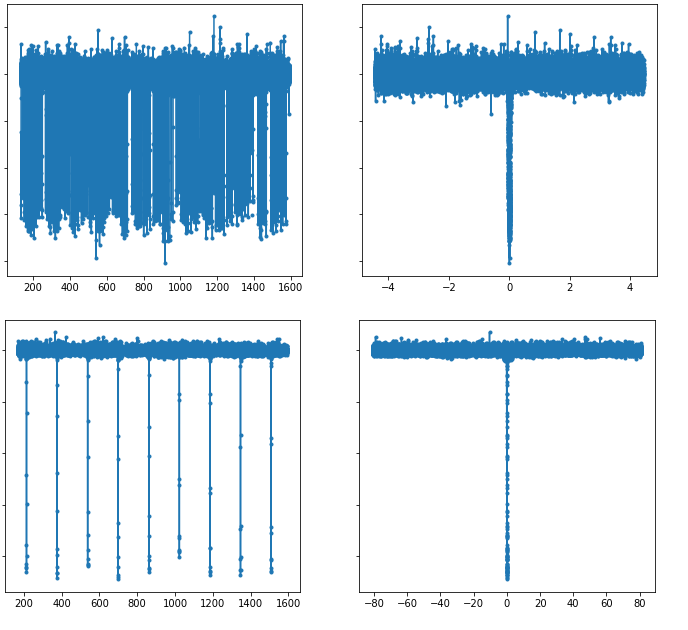
\includegraphics[width=0.95\textwidth, height=8cm]{imgs/LC_ex.png}
%    \caption{Examples of light curves on Kepler mission. First column correspond to 4 years measurements with sampling rate of half an our, while the second column correspond to the isolated transit.}
%    \label{fig:lc_ex}
%\end{figure}


%\subsection{Representation}

We assume that the time series measurements are median-centered and that the main variations are from the transients. Therefore, the values of interest are the negative transitions. We re-scale every light curve $x^{(\ell)}$ so that the $T_{\ell}$ measurements fall into $[-1,1]$ \citep{shallue2018identifying}. Based on the assumptions, the process is given by:
\begin{equation} \label{rep:pre}
    x_{t}^{(\ell)} = \frac{x_{t}^{(\ell)}}{min(x^{(\ell)})} \ , \ \ \forall t
\end{equation}


\subsection{Constructing the MTF}
\begin{algorithm}[!t] 
\caption{Light Curve to MTF}
\label{alg:lc_to_mtf}
\hspace*{\algorithmicindent} \textbf{Input}: $x^{(\ell)}$ - light curve measurements ($T_{\ell}$-dimensional vector) \\
\hspace*{\algorithmicindent} \hspace{0.1\textwidth} $s^{(\ell)}$ - light curve timestamp ($T_{\ell}$-dimensional vector) \\
\hspace*{\algorithmicindent} \hspace{0.1\textwidth} $n_{up}$ - number of states in positive values \\
\hspace*{\algorithmicindent} \hspace{0.1\textwidth} $n_{down}$ - number of states in negative values \\
\hspace*{\algorithmicindent} \hspace{0.1\textwidth} $\delta_T$ - maximum delta time \\ %tiempo pepe
\hspace*{\algorithmicindent} \textbf{Output}:  $M$ - MTF ($N \times N$ matrix)
\begin{algorithmic}[1]
\State $N \gets n_{up}+ n_{down}$  %N
\State $M \gets $ empty$(N, N)$
\State $S_{grid} \gets $ states\_grid$(n_{up},n_{down})$ \ //list of interval states
\For {observation $t \in \{1,2, \ldots, T_{\ell}-1\}$}
    \State $delta \gets s^{(\ell)}_{t+1}-s^{(\ell)}_t$
    %\If{$\mid  delta - \delta_T  \mid \leq \epsilon $ }
    \If{$  delta \leq \delta_T + \epsilon $ }
        %\State //Add state transitions count
        \State $i \gets $ detect\_state$(x^{(\ell)}_{t},S_{grid})$
        \State $j \gets $ detect\_state$(x^{(\ell)}_{t+1},S_{grid})$
        \State $M_{i,j} \gets M_{i,j} + 1$ \ //add state transitions count
    %\Else{}
    %    \State continue
    \EndIf
\EndFor
%\State 
\For {state $i \in \{1,2, \ldots, N\}$}  %N
    %\State $count_i \gets sum(M_{i,\cdot})$
    \State $M_{i,\cdot} \gets M_{i,\cdot}/ sum(M_{i,\cdot})$ \ //normalize probabilities  %   count_{i}$ 
\EndFor
\end{algorithmic} 
\end{algorithm}

%\documentclass[margin=0.5cm]{standalone}
%\usepackage{tikz}
%\usetikzlibrary{matrix,decorations.pathreplacing,calc,fit}

\pgfkeys{tikz/mymatrixenv/.style={decoration=brace,every left delimiter/.style={xshift=4.7pt},every right delimiter/.style={xshift=-4.7pt}}}
\pgfkeys{tikz/mymatrix/.style={matrix of math nodes, nodes in empty cells, left delimiter=[,right delimiter={]},inner sep=2pt,column sep=1em,row sep=0.5em,nodes={inner sep=0pt}}}
\pgfkeys{tikz/mymatrixbrace/.style={decorate,thick}}

% The hack required for foreach loops in fit. Code from https://tex.stackexchange.com/questions/4751/fitting-a-list-of-points-with-tikz-and-its-foreach?noredirect=1&lq=1
\makeatletter
\def\tikz@lib@fit@scan{%
  \pgfutil@ifnextchar\pgf@stop{\pgfutil@gobble}{%
    \pgfutil@ifnextchar\foreach{\tikz@lib@fit@scan@handle@foreach}{%
      \tikz@scan@one@point\tikz@lib@fit@scan@handle}}}
\def\tikz@lib@fit@scan@handle@foreach\foreach#1in#2#3{%
  \foreach #1 in {#2}
  {\tikz@scan@one@point\tikz@lib@fit@scan@handle@foreach@#3}
  \tikz@lib@fit@scan}
\def\tikz@lib@fit@scan@handle@foreach@#1{%
  \iftikz@shapeborder
    \tikz@lib@fit@adjust{%
      \pgfpointanchor{\tikz@shapeborder@name}{west}}%
    \tikz@lib@fit@adjust{%
      \pgfpointanchor{\tikz@shapeborder@name}{east}}%
    \tikz@lib@fit@adjust{%
      \pgfpointanchor{\tikz@shapeborder@name}{north}}%
    \tikz@lib@fit@adjust{%
      \pgfpointanchor{\tikz@shapeborder@name}{south}}%
  \else
    \tikz@lib@fit@adjust{#1}%
  \fi
  \global\pgf@xa=\pgf@xa
  \global\pgf@ya=\pgf@ya
  \global\pgf@xb=\pgf@xb
  \global\pgf@yb=\pgf@yb}
\makeatletter

%\begin{document}

\begin{figure}[!t]
    \centering
    %\includegraphics{}
    
\begin{tikzpicture}[baseline=0cm,mymatrixenv]
    \matrix [mymatrix,outer ysep=0.7pt,inner sep=4pt,row sep=1em] (m)  
    {
    m_{1,1}  &  m_{1,2} &  m_{1,3} & m_{1,4} & m_{1,5} &  m_{1,6} & \dots & m_{1,n}  \\
    m_{2,1}  &  m_{2,2} &  m_{2,3} & m_{2,4} & m_{2,5} &  m_{2,6} & \dots & m_{2,n}  \\
    m_{3,1}  &  m_{3,2} &  m_{3,3} & m_{3,4} & m_{3,5} &  m_{3,6} & \dots & m_{3,n}  \\
    m_{4,1}  & m_{4,2} & m_{4,3} & m_{4,4} & m_{4,5} & m_{4,6} & \dots & m_{4,n} \\
   m_{5,1}   & m_{5,2} & m_{5,3} & m_{5,4} & m_{5,5} & m_{5,6}  & \dots & m_{5,n} \\
    m_{6,1}  & m_{6,2} & m_{6,3} & m_{6,4} & m_{6,5}  & m_{6,6} & \dots & m_{6,n}\\
    \vdots   & \vdots  & \vdots  & \vdots  & \vdots  & \vdots  & \ddots & \vdots \\
    m_{n,1}  & m_{n,2} & m_{n,3} & m_{n,4} & m_{n,5} & m_{n,6} & \dots & m_{n,n} \\
    };

% Colours
\definecolor{brightpurple}{HTML}{C151EF}

\node [fit= \foreach \X in {1,...,3}{(m-\X-1)}
            \foreach \X in {1,...,3}{(m-\X-2)}
            \foreach \X in {1,...,3}{(m-\X-3)}]
            [draw=green, thick,inner sep=2.6pt] (fit-a) {};

\node [fit= \foreach \X in {4,...,6}{(m-\X-4)}
            \foreach \X in {4,...,6}{(m-\X-5)}
            \foreach \X in {4,...,6}{(m-\X-6)}]
            [draw=cyan, thick,inner sep=2.6pt] (fit-b) {};

\node [fit= \foreach \X in {2,...,4}{(m-\X-2)}
            \foreach \X in {2,...,4}{(m-\X-3)}
            \foreach \X in {2,...,4}{(m-\X-4)}]
            [draw=orange, thick,inner sep=2.6pt] (fit-c) {};
            
\node [fit= \foreach \X in {3,...,5}{(m-\X-3)}
            \foreach \X in {3,...,5}{(m-\X-4)}
            \foreach \X in {3,...,5}{(m-\X-5)}]
            [draw=purple, thick,inner sep=2.6pt] (fit-d) {};
            
% FINDING VERTICAL MIDPOINT
 \node [fit= \foreach \X in {1,...,3}{
            (m-\X-1)}] (fit-one)  {}; 
 \node [fit= \foreach \X in {4,...,6}{
            (m-\X-6)}] (fit-two)  {}; 
\path (fit-one.south) -- (fit-two.north) coordinate[midway] (X);

% FINDING HORIZONTAL MIDPOINT
 \node [fit= \foreach \X in {1,...,3}{
            (m-1-\X)}] (fit-one)  {}; 
 \node [fit= \foreach \X in {4,...,6}{
            (m-6-\X)}] (fit-two)  {}; 
\path (fit-one.east) -- (fit-two.west) coordinate[midway] (Y);

\newcommand\mymatrixbraceoffseth{0.3em}
\newcommand\mymatrixbraceoffsetv{0.3em}

% LHS BRACES
\draw [mymatrixbrace] ($(m.north west)!(fit-a.south)!(m.south west)-(\mymatrixbraceoffseth,0)$)   -- node[left=3pt] {$K_1$}  ($(m.north west)!(fit-a.north)!(m.south west)-(\mymatrixbraceoffseth,0)$);
\draw [mymatrixbrace] ($(m.north west)!(fit-b.south)!(m.south west)-(\mymatrixbraceoffseth,0)$) -- node[left=3pt] {$K_2$} ($(m.north west)!(fit-b.north)!(m.south west)-(\mymatrixbraceoffseth,0)$);

% TOP BRACES       
\draw[mymatrixbrace] ($(m.north west)!([xshift=0.05cm]Y)!(m.north east)+(0,\mymatrixbraceoffsetv)$) -- node[above=3pt] {$K_2''$}  ($(m.north west)!(fit-b.east)!(m.north east)+(0,\mymatrixbraceoffsetv)$);
\draw[mymatrixbrace] ($(m.north west)!(fit-a.west)!(m.north east)+(0,\mymatrixbraceoffsetv)$)-- node[above=3pt] {$K_1'$}   ($(m.north west)!([xshift=-0.05cm]Y)!(m.north east)+(0,\mymatrixbraceoffsetv)$);

\end{tikzpicture}
\caption{Illustration of a Markov Transition Field (MTF) matrix. Each entry into the matrix ($m_{i, j}$) corresponds to a defined state. Each box corresponds to a feature map for a $3 \times 3$ kernel size.}
\label{fig:matrix_MTF}
\end{figure}


%\end{document}

\begin{figure}[!t]
    \centering
    \subfloat[Light measurements transitions.]{{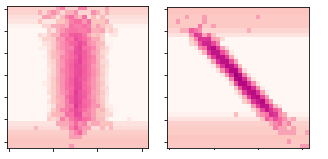
\includegraphics[width=0.45\textwidth]{imgs/MTF_lc_ex.png} }}%
    \qquad
    \subfloat[Time transitions.]{{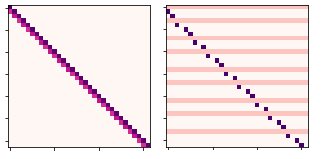
\includegraphics[width=0.45\textwidth]{imgs/MTF_time_ex.png} }}%
    \caption{Image representation (MTF) for light curve transitions (the measurements and the time) by using $n_{up}=n_{down}=16$ states ($32\times 32$ matrix). Examples are from light curves on the Kepler mission.}%
    \label{fig:mtf_ex:prop}
\end{figure}


A Markov Transition Field $M$ \citep{wang2015imaging} for a time series $x^{(\ell)}$ is constructed by taking all the continuous numerical values from $x_1^{(\ell)}$ to $x_{T_{\ell}}^{(\ell)}$. The meaning of a transition probability $m_{ij}$ in $M$ can be interpreted as the likelihood of transition from state $i$ to $j$ where $i,j \in N$. 
How to build this transition matrix for irregular sampled time series is not clear. We propose to take in consideration all the \textit{semi-continuous} (continuous over a maximum delta time) transitions to count the frequency and generate the probabilities with the relative frequency as \citep{wang2015imaging} propose. 
Thus, the probabilities $m_{ij}$ are built based on the number of \textit{semi-continuous} transitions from state $i$ to state $j$ (absolute frequency) normalized by the number of transitions from state $i$.
A pseudo-code to illustrate this for a $\ell$ time series is presented in Algorithm \ref{alg:lc_to_mtf}, where the main inputs are the measurements $x^{(\ell)}$ and timestamps $s^{(\ell)}$.
The maximum delta time to consider the \textit{semi-continuous} transitions ($\delta_T$) need to be defined too. It must be defined depending on the dataset behavior. In our case, we set it according the Kepler sampling rate (half of an hour).
%como conenctar con lo anterior??
First, we define a linear grid over the $[-1,1]$ interval to represent the states. We set different numbers for positive measurements $[0,1]$ (with $n_{up}$ values) and for negative measurements $[-1,0]$ (with $n_{down}$ values), this is the line 3 of the pseudo-code (i.e, ``states\_grid" function).
The number of intervals in positive and negative values could be manually defined in order to obtain more tailored transitions for each application while the ``detect\_state" function on line 7 and 8 finds the corresponding state for a specific measurement $x_t^{\ell}$ on the defined grid and
the line 6 is crucial, since it performs the \textit{semi-continuous} check of the transitions. 
Figure \ref{fig:mtf_ex:prop} shows examples of the final MTF matrix for the light curves observations.

Finally, $M$ has a dimension of $N \times N$, with $N=n_{up}+n_{down}$. In that sense, for convolutional neural networks \citep{krizhevsky2012imagenet}, a window of $k$ states represent the feature map that is fed to the model. So the feature map consider $k$ consecutive states from $M$, as Figure \ref{fig:matrix_MTF} shows.

%In addition, with the propose of use the irregular sampled time information, we build a time transitions matrix, described below.

\subsection{Constructing Time Transitions}
\begin{figure}[t!]
\centering
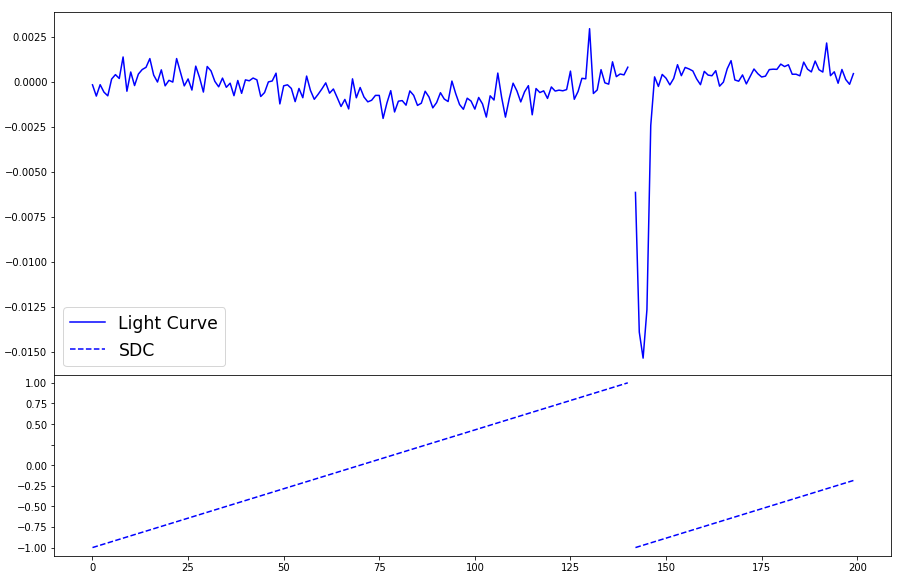
\includegraphics[width=0.85\linewidth, height=5cm]{imgs/sdc.png}
\caption{SDC from light curve. At the top image shows a sequence of 200 measurements from a given light curve; At the bottom is the SDC for the sample. Note that SDC is normalized in order to be consistent with the scale that the light curve has.}
\label{fig:sdc_example}
\end{figure}
To create the time channel for the image representation, we generate a \textit{Sample Detection Curve} (SDC) which maintains a sequence of counts of valid \textit{semi-continous} measurements based on a specific delta time, $\delta_T$. If two consecutive measurements have a timestamp difference greater than $\delta_T$, the count will restart. In this way, SDC provides information about the time transitions of a light curve. 
Algorithm \ref{alg:lc_to_sdc} shows how the SDC is build from the timestamps $s^{(\ell)}$ of a $\ell$ light curve considering a maximum delta time for \textit{semi-continuous} transitions ($\delta_T$).
Figure \ref{fig:sdc_example} shows a visual example of the SDC for a light curve.

\begin{algorithm}[t!] 
\caption{Light Curve to SDC}
\label{alg:lc_to_sdc}
\hspace*{\algorithmicindent} \textbf{Input}: $s^{(\ell)}$ - light curve timestamp ($T_{\ell}$-dimensional vector) \\
\hspace*{\algorithmicindent} \hspace{0.1\textwidth} $\delta_T$ - maximum delta time \\ 
\hspace*{\algorithmicindent} \textbf{Output}:  $SDC$ - semi continuous information ($T_{\ell}$-dimensional vector)
\begin{algorithmic}[1]
\State $SDC \gets empty(T_{\ell})$  //empty list of size $T_{\ell}$
\State $SDC[1] \gets 0$  //start of the sequence
\State $count \gets 1$
\For {observation $t \in \{1,2, \ldots, T_{\ell}-1\}$}
    \State $delta \gets s^{(\ell)}_{t+1}-s^{(\ell)}_t$
    \If{$\mid  delta - \delta_T  \mid > \epsilon $ }
        \State $count \gets 0 $ //reset count
    \EndIf
    \State $SDC[t+1] \gets count $
    \State $count \gets count + 1 $
\EndFor
\State $SDC \gets \frac{SDC - min(SDC)}{ max(SDC) -min(SDC)} $ // re-scale into [0,1]
\State $SDC \gets 2 \cdot SDC - 1$ // re-scale into [-1,1]
\end{algorithmic}
\end{algorithm}
Based on the re-scaled SDC (into $[-1,1]$ range) we can build the MTF of that information in the same way for light curve measurements.
The main idea is to apply Algorithm \ref{alg:lc_to_mtf} with the same number of states and maximum delta, but replacing the light curves measurements $x^{(\ell)}$ with the corresponding SDC.
Figure \ref{fig:mtf_ex} shows examples of the time channel on the final image representation (MTF), where it can be seen different sampling time patterns of the observation.



%\subsection{Number of States Effect}
%The number of states have a trade-off between a fine-grained (detailed) and a coarse (compressed) representation. A higher number of states will create a detailed fine-grained representation but sparser (with only a few transitions for each state). While a low number of state will group some states having a less detailed representation but denser (with more transitions for each state). Also it is complicated when it comes to define how many states on the positives ($n_{up}$) and on the negatives ($n_{down}$) values. For example, in order to have a more simpler and symmetric structure, we could define the same number of states for positive and negatives values. While if we want a matrix with more detailed transitions on the transits (blocking star light) the number of negatives states ($n_{down}$) has to be higher than the number of positives states ($n_{up}$). However, if we want a matrix with more detailed transitions on the out-of-shelf factors (e.g. background noise, astronomical objects or phenomenon) the $n_{up}$ value has to be higher than $n_{down}$.




\section{Experimental Setup}
\label{exp}

\subsection{Dataset}
%no hablar mucho de etiquetas puesto que es solo para evaluacion... es una tecncia no supervisada.
%Currently, the dataset with the most studied exoplanets is from the NASA based on the effectiveness of Kepler mission\footnote{Kepler measured the light variation of thousand of distant stars in search of periodic planetary transit within our galaxy neighborhood.}. Particularly,

Our work uses the \textit{Kepler Objects of Interest} (KOI) dataset\footnote{http://archive.stsci.edu/search\_fields.php?mission=kepler\_koi} provided by MAST (\textit{Mikulski Archive for Space Telescopes}) \citep{akeson2013nasa}. It is composed by 8054 records where every Kepler Object of Interest (KOI) is a region of interest in the sky that shows a periodic behavior based on thresholding events. These objects are categorized according to Nasa Exoplanet Science Institute\footnote{http://nexsci.caltech.edu/}, as \textit{Confirmed}, claimed exoplanets through extensive scientific analysis and follow ups; \textit{False Positive}, initially selected as candidate exoplanets but additional evidence show they are not; or \textit{Candidate}, those that are still under study (unlabeled data).
Multiple KOIs are obtained from each host star, and each object contains raw measurements with timestamps, including the instrumental error associated to each measure. The sampling rate is 0.0204 BJD on average (i.e., half an hour), but there is a 22.98\% of missing values per light curve on average. Each light curve has approximately 55000 effective measurements.

The archive also provides a set of metadata values, some of them (usually related to the star) are cross-matched from other catalogues. For comparing our self-generated features with model-based ones, we have selected only those that can be directly obtained from the light curves by following the Mandel-Agol model \citep{mandel2002analytic}.
%\emph{period}, \emph{First Transit Time}

%\subsubsection*{\textbf{Metadata}}
%From all the high-level features (metadata) that was available, we have selected the features that can be extracted only from the light curve, without cross-matching from other cataloges.
%\begin{itemize}
%\item \emph{Period}: the interval between consecutive planetary transits in days. Calculated as one of the best-fit parameter on a Mandel-Agol model \citep{mandel2002analytic}.
%\item \emph{First Transit Time}: the time when the exoplanet pass in front of the host star in BJD. Calculated as one of the best-fit parameter on a Mandel-Agol model \citep{mandel2002analytic}.
%\item \emph{Inclination}: the angle between the plane of the sky (perpendicular to the line of sight) and the orbital plane of the object (90 degrees is a orbit in the line of sight). Calculated as one of the best-fit parameter on a Mandel-Agol model \citep{mandel2002analytic}.
%\item \emph{Planet Radius} (over Stellar Radius): the inferred radius of the Object of Interest. Based on a best-fit parameter on a Mandel-Agol model \citep{mandel2002analytic}. Calculated as one of the best-fit parameter on a Mandel-Agol model \citep{mandel2002analytic}.
%\item \emph{Semi-major Axis} (over Stellar Radius): orbital radius based on the axis of an elliptic orbit. Calculated as one of the best-fit parameter on a Mandel-Agol model \citep{mandel2002analytic}.
%\item \emph{Limb Darkening Coefficients}: models the light variation (darkening) on the edges of the star, two coefficient (linear and quadratic). To be sure, Kepler used cross-matching.

%\item \emph{Impact Parameter}: distance between the object and the sight axis to the star. Calculated based on the orbit radius and the inclination.
%\item \emph{Transit Duration}: time between first contact and last contact in days (eclipse duration). Calculated based on the transit period, planet radius and orbit radius.
%\item \emph{Fitted stellar density}: calculated based on a small planet approximation with the planet radius, transit period and duration.
%\item \emph{Planet Teq}: the expected temperature of equilibrium on the surface of the candidate planet in Kelvin. Calculated through the stellar temperature and the planet's radiation.
%\end{itemize}


%\subsection{Dataset Pre-processing}
We use Kepler's detrend pipeline \citep{fanelli2011kepler} to obtain a standard light curve for our experiments, i.e. that express the changes respect to a local window behavior. It consist on applying
%\begin{enumerate}
%    \item Apply 
a polynomial fit, Sav-Gol filter \citep{savitzky1964smoothing}, of 2 degrees with a window of 151, and then subtract it to the light curve. Then it
   % \item Apply  and 
subtracts a moving median filter, with a window of 25.
Finally, we removes
%    \item Remove 
positive outliers that are high than $5\sigma$ and removes negative outliers lower than $40 \sigma$. 
%With $\sigma$ the standard deviation of the light curve.
%\end{enumerate}


\subsection{Data Representation}
\begin{figure}[!t]
    \centering
    \begin{tabular}{c}
        Example 1 \\
         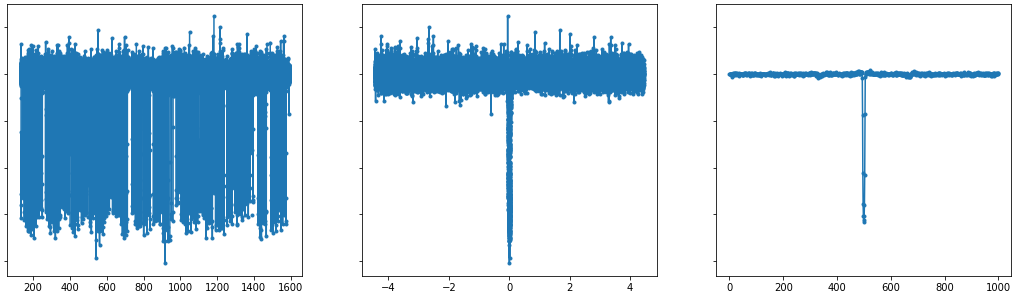
\includegraphics[width=0.95\textwidth, height=3cm]{imgs/conf_ex.png}  \\
        Example 2 \\ 
         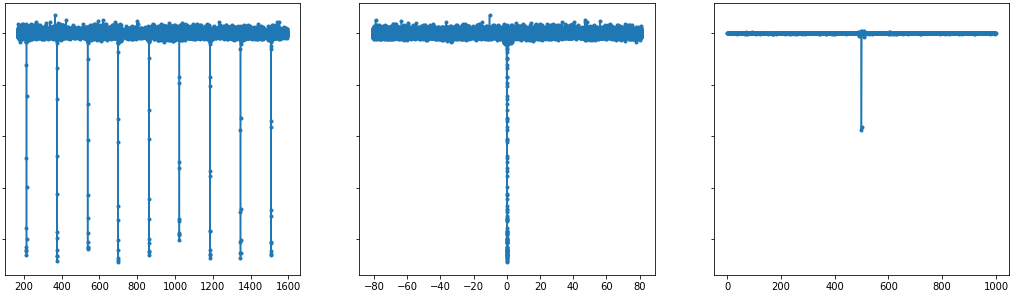
\includegraphics[width=0.95\textwidth, height=3cm]{imgs/narrow_ex.png} \\
         Example 3 \\ 
         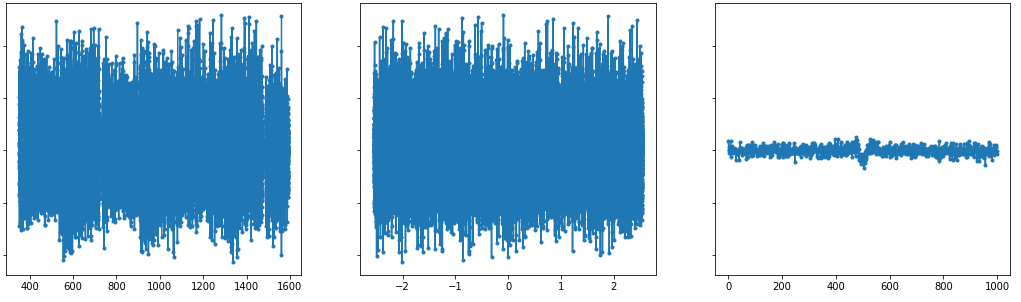
\includegraphics[width=0.95\textwidth, height=3cm]{imgs/noisy_ex.png} 
    \end{tabular}
    \caption{Examples on the different representation that can be obtained from a periodic light curve by knowing the period $P$. The images on every example is the raw light curve, the folded and folded-global (setting the bins to $T=1000$) on the columns respectively. The third column is the representation used on this work.}
    \label{fig:representation_ex}
\end{figure}

For the light curve measurement $x^{(i)}$, we use the \textbf{folded-global} representation proposed by \citep{shallue2018identifying}. First it produce a vector $f^{(i)}$ with the same number of points by folding the raw light curve on the period ($P$), with the event centered (fold step). Then, a windowed median is applied every $P/T$ times over the folded light curve $f^{(i)}$ (global step). This produces a vector $\mathbf{x}^{(i)}$ with $T$ points, so each light curve has the same length with the width interval depending on the period $P$.
%This representation was original used to classify \textit{Thresholding Crossing Event} (TCE)\footnote{This is detect Candidates from False Positive objects} with a good performance. The process is described here:
%\begin{enumerate}
%    \item \textit{Fold}: Produce a vector $f^{(i)}$ with the same number of points by folding the raw light curve on the period ($P$), with the event centered (need the \textit{first time transit} measure).
%    \item \textit{Global}: A window median is applied every $P/T$ times, on the folded light curve $f^{(i)}$. Producing a vector $\mathbf{x}^{(i)}$ with $T$ points, so each light curve has the same length with the width interval depending on the period $P$.
%\end{enumerate}
The parameter $T$ controls the trade-off between a detailed representation and having enough points on each window for the median to be meaningful.

Figure \ref{fig:representation_ex} shows examples of folded and folded-global representations of light curves.
The second example illustrates a general disadvantage of this method, where long-period KOIs may end up with very narrow transits that fall entirely within a small number of bins. On the other hand, the third example shows how the folded-global representation helps to get a more cleaned version of the light curve when the planets are small. 

As explained in Section~\ref{proposal}, the delta times ($\delta^{(i)}$) of the folded-global representation are considered as an additional input for the learning models. 
Also, please recall that the light curve measurements $\mathbf{x}^{(i)}$ are previously normalized through $\mathbf{x}'^{(i)} = \mathbf{x}^{(i)}/std(\mathbf{x}^{(i)})$ for VRAE$_t$,%, as pre-process let the light curves centered ($mean(\mathbf{x}^{(i)}) = 0 \ \forall i$). 
while the raw light curve measurements $\mathbf{x}^{(i)}$ are used for the proposed S-VRAE$_t$ model.


\subsection{Data Selection and Augmentation} %and Further Processes
%We set a mask over all the objects on Kepler mission (8054 records) to filter out light curves without a transit behavior, obtaining 4317 objects to train our models. 
%Concretely, we remove objects that either (i) are classified as ``secondary transit" or ``not transit", (ii) have a \textit{transit score} lower than $0.55$, or (iii) have a Mandel-Agol residual higher than $1$.
%The candidates objects that are not transit could be because the transit was from another object (non-planetary) in the background or because it was a binary system, i.e. two stars orbiting around their barycenter.

We set a mask over all the objects on Kepler mission (8054 records) to filter out light curves without a transit behavior, obtaining 4317 objects to train our models. The process is described below:
\begin{itemize}
    \item Check for Kepler \textit{flags} (metadata) and remove objects with ``secondary transit" or ``not transit" flags.
    \item Check for \textit{transit score} (Kepler metadata) and remove objects with value lower than $0.55$.
    \item Perform a Mandel-Agol fit and check the residual, remove the object with \textit{SMSE} higher tan $1$.
\end{itemize}
%Between the reason to set the flags on the Kepler pipeline we found that the observation did not match with the star position on study, for instance because the transit was from another object (non-planetary) in the background (``not transit" flag).
%Another possibility is that the deep of the even transit was statistically different to the deep of the odd transits, showing a binary system, i.e two stars orbiting among them (``secondary transit" flag).
The candidates objects that are not transit could be because the transit was from another object (non-planetary) in the background (``not transit" flags) or because it was a binary system, i.e. two stars orbiting around their barycenter, so it has a second statistically different transit (``secondary transit" flag).

Also, as a data augmentation step \citep{tiensuu2019detecting}, we double this dataset by mirroring each folded light curve. This represents that the same object, with the same properties, orbits the star in the opposite direction. 


\subsection{Model Implementation}
Following the RAE$_t$ model \citep{naul2018recurrent}, our VRAE and VRAE$_t$ models implement GRU over LSTM on the recurrent layers as it presents roughly the same performance \citep{chung2014empirical}, but has fewer parameters and needs to store less information per time series (i.e., it is faster). The encoder and decoder recurrent section of the models (i.e., $E^1$ and $g^1$ on Algorithms \ref{alg:vrae} and \ref{alg:s-vrae}) are a stack of 2 bidirectional RNN layers of 64 units, in order to increase representation complexity as \citep{naul2018recurrent} present. We implement our model using the Keras library\footnote{\texttt{https://keras.io}}.   %codigo


\subsection{Model Assessment}

%test seT???

\subsubsection*{Encoder-Decoder Evaluation} %AE/VAE

For assessing the \textit{reconstruction} quality, we compare the estimated input pattern $\hat{x}$ and real value $x$, using the Root Mean Squared Error (\textbf{RMSE}) and Mean Absolute Error (\textbf{MAE}) as performance metrics. For evaluating the \textit{denoising} effect, we use the estimated input pattern $\hat{x}$ to measure the autocorrelation (\textbf{Autocorr}) and the Mean of the Differences (\textbf{Diff-M}) between consecutive values. A high autocorrelation and low mean difference, is associated to a smoother time series. For measuring the structure left within the \textit{residual noise} (difference between estimated and real input pattern), we use
%Based on the residual of model outputs, i.e. difference between estimated input pattern $\hat{x}$ and real value $x$. A 
an information theory score called the Spectral Entropy (\textbf{Spectral-H}) \citep{inouye1991quantification}. A high entropy value means a less structured residual in terms of signal frequencies.

Smoothing a time series is a classical signal processing task, but unfortunately this is not straightforward for transits, because transits are (statistically speaking) isolated behaviors or anomalies (i.e., threshold events) as Figure \ref{fig:representation_ex} shows. Therefore, a \textit{vanilla} denoising model will remove transits by considering them anomaly deviations of the ``normal'' star magnitude.
Based on this, we have selected the following baselines to compare our models: the Butterworth passband filter \citep{chandrakar2013survey}, a moving average filter with different window size, a Mandel-Agol simulation based on the object metadata and the Recurrent Auto-Encoder plus time (RAE$_t$) by \citep{naul2018recurrent} .

\subsubsection*{Encoder evaluation} %deep representation
For evaluating the deep representation quality learned by the encoder sub-architecture, we analyzed how it performs in a classification task, and how orthogonal the generated features are.
The \textit{classification} was made using a Feed Forward (FF) network built over the representation with 128 units and \textit{relu} activation, ending with a \textit{sigmoid} classification layer (1-unit) as output. The model is trained using the dataset labels (2281 exoplanets and 3976 non-exoplanets). A F1 macro criterion (\textbf{F1-Ma}) is used to assess the results. 

For analyzing the \textit{features dependence} a Pearson correlation between all the features on the representation was measured to find linear dependence. We report the average over all the values (\textbf{Pcorr}) and the average over the absolutes values (\textbf{Pcorr-A}).  
The Mutual Information between the continuous features is measured as well (\textbf{MI}), including a normalized version (value between $[0,1]$) that is obtained by dividing on the entropy of every feature (\textbf{N-MI}). The calculation of Mutual Information is a discrete approximation of the real continuous space calculation, based on the $k$-neighbors implementation \citep{ross2014mutual}.
    %\item \textit{Clustering}: ??
    %\item \textit{Interpretability}: Pendiente

Here we compare with the high-level specialized features included in Kepler's metadata, the features learned by a Recurrent Auto-Encoder plus time (RAE$_t$) \citep{naul2018recurrent}, and the PCA features extracted over the frequency domain (spectrum) representation of the time series (F+PCA) \citep{bugueno2018refining}. 


%Decoder using:
%para generar curvas y agregar interpretabilidad

\section{Results}
The results of our experiments were obtained thanks to the ChiVO\footnote{\texttt{https://chivo.cl/}} (Chilean Virtual Observatory) datacenter \citep{solar2015chilean} by using an Intel Xeon CPU E5-2680 2.50GHz with 12 cores and 64 GB of RAM.

\subsection{Number of States Impact}
\begin{table}[!t]
    \caption{Macro averaged F1-score on validation set for different number of settings. $n_{up}$ stands for the number of positive states while $n_{down}$ corresponds to negative states defined for the MTF representation. $*$ symbol shows the best result.}
    \label{tab:exp_states}
    \centering
    \begin{tabular}{c|ccccc}
        \diaghead(-2,1){\hspace{1.7cm}}{$n_{up}$}{$n_{down}$}& %do not change
            8 & 16 & 32 & 64 \\ \hline
        4  & 71.48 & 72.66 & 72.97 & 71.81 \\ 
        8  & 72.14 & 73.35 & 74.43 & 72.00 \\ 
        16 & 72.84 & 74.69 & 75.75$^*$ & 74.13  \\ 
        32 & 73.84 & 75.03 & 75.40 & 75.53 \\  
        64 & 72.75 & 73.47 & 74.03 & 74.95  \\ 
        \hline
        %128 & $\times$ & $\times$ & $\times$ & $\times$ & $\times$ %& Si
    \end{tabular}
\end{table}
Table \ref{tab:exp_states} presents the experimental impact of the number of states in the classification task. 
The best \textit{F1-score} was obtained by using $n_{up} = 16$ and $n_{down}=32$, which is a 2-channel image of $48\times 48$ size.
Note that as the number of states increases (both $n_{up}$ and $n_{down}$), the performance improves, this is because the model input becomes a fine-grained representation (more detailed image).  
However, for any $n_{up}$ up to 16 states, macro averaged \textit{F1-score} reaches a maximum with $n_{down}=32$, then it decays. %(with $n_{down}=64$). 
The experimental results show that the number of transitions does not need a more fine-grained representation ($n_{down} \geq 64$) because the transit information turns fuzzy, so each pixel of the image does not represent aggregated information. In that sense, the MTF image results in a very sparse matrix, since there is a lot of states but only a few transitions per state. 

By using $n_{up}=32$ or $n_{up}=64$, when more $n_{down}$ states are used a higher \textit{F1-score} is reached.
This shows that the positive-negative symmetric states, i.e. $n_{up}=n_{down}$, are not always the best setting.
Most of the cases reach better results when a higher number of states on the negative values is set.
Indeed, given an $n_{up}$, the number of negative states ($n_{down}$) should be higher or equal to $n_{up}$. 
This makes sense if we analyze the problem context since the negative transitions (light blocking) are more important than the positive ones (noise and stellar properties).

\subsection{Method Comparison}
Using the best setting on validation set, $48\times 48$ images ($n_{up} = 16 $ and $n_{down} = 32$), we obtain the final results on the test set against the compared methods.

\begin{table}[!t]
\caption{Classification performance using different methods and feature extraction techniques. The \textit{F1-score} per class (C: \textit{Confirmed}, FP: \textit{False Positive}) and the macro averaged \textit{F1-score} are presented. $\star$ The feets results reported corresponds to a sample of 2500 objects (2 months execution).}
\label{tab:class_results}
\begin{tabular}{c|c|cc|c} \hline
\textbf{Method} & \textbf{Input shape} & \textbf{FP class}& \textbf{C class} & \textbf{Macro avg.} \\ \hline 
\multicolumn{5}{c}{\textit{Specialized hand-crafted features + Classic Learning Methods}} \\ \hline
Metadata  & $10$                 & $90.13$ & $83.85$  & $87.00$ \\ %\hline
feets$^{\star}$     & $57$                 & $84.57$ & $31.19$  & $57.88$    \\ \hline
\multicolumn{5}{c}{\textit{Feature extraction + Classic Learning Methods}} \\ \hline
F-PCA  & $32$                 & $80.03$ & $58.54$  & $69.29$ \\ \hline
%fourier + ica??
\multicolumn{5}{c}{\textit{Deep Learning Methods}} \\ \hline
1D CNN raw  & $70000\times 2$         & $84.43$ & $67.68$ & $76.06$  \\ 
\textbf{2D CNN MTF} 
            & $48\times48\times 2$    & $84.26$   & $69.76$  & $77.01$   \\ 
\hline
%poner folded? yo diria que no .. ya que les va muy bien jaja y enrealidad hacen trampa al conocer el periodo.. (si se sabe el periodo mejor usar la metadata)
\end{tabular}
\end{table}
Table \ref{tab:class_results} compares different methods according to \textit{F1-score} metric.  %remarked in baseline section for the exoplanet detection problem by \textit{F1-score}. 
The classification for classic learning was made using the fully connected block of deep architectures (Table \ref{tab:model:arch}). This corresponds to 128 dense units with \textit{relu} activation function followed by the classification dense layer with one unit and \textit{sigmoid} activation function. 
Firstly, our method obtains a moderate F1-score macro averaged improvement of 0.95 over a 1D CNN, despite of the 1D CNN method uses a fairly sophisticated architecture with a large number of parameters (Table \ref{tab:model:arch}).
Drawing on 2D CNN model, our method extracts enough information to identify transit patterns on the MTF images.

Deep learning methods outperform the classic counterpart approach of F-PCA by $\sim 8\%$ and the hand-crafted features of feets showing a large gap ($\sim 33\%$). 
However, the specialized features for the problem, metadata, have the best performance for the task. 
Note that our method reaches the second best result, meaning that still are some improvements that could be done with the automatic techniques.

The detailed metrics per class show that the confirmed class is the most difficult to detect, meaning that the behavior of the exoplanets is not so clear in order to group and discriminate correctly all the patterns. 
The advantage from the metadata representation comes from this class, showing large improvement against all the other methods. 
The false positive class (non-exoplanets) appears easier to detect, based on the \textit{F1-score} higher than 80\% for all the methods. 
%While the false positives class (non-exoplanets) appears more easier to detect based on the probably clear patterns of the binary system or noise properties.

\begin{table}[!t]
\caption{Time comparison in seconds for different learning techniques. Values in parenthesis on Training column stands for the number of epochs to train the models. $\diamond$ This value is based on the information of \citep{fanelli2011kepler}, this is 4 days. $\star$ The feets representation time is measured over a subset of 2500 objects (30\% of the data).}
\label{tab:time_results}
\begin{tabular}{c|ccc|c} \hline
\textbf{Method} & \textbf{Representation} & \textbf{Training} & \textbf{Predict} & \textbf{Total} \\ \hline 
\multicolumn{5}{c}{\textit{Specialized hand-crafted features + Classic Learning Methods}} \\ \hline
Metadata   & $5760^\diamond$ & $37.8$ (200)  & $0.04$ & - \\ %\hline
feets      & $5912500^{\star}$   & $42.2$ (200)  & $0.07$ & $>100000$ mins \\ \hline %($2365$ x D)
\multicolumn{5}{c}{{\textit{Feature extraction + Classic Learning Methods}}} \\ \hline
F-PCA          & $166.6$  & $40.4$ (200) & $0.06$ & $\sim$ 4 mins \\ \hline  %\hline %$96.6$ (Fou) $0.012$ x D , $70$ (PCA
\multicolumn{5}{c}{{\textit{Deep Learning Methods}}} \\ \hline
1D CNN raw             & $0$ & $21500$ (50)  & $288.33$ & $\sim$ 360 mins  \\ 
\textbf{2D CNN MTF} 
                       & $145$ & $1040$ (200) & $4.72$ & $\sim$ 20 mins \\ %($0.018$ x D)
\hline
\end{tabular}
\end{table}
Table \ref{tab:time_results} shows the execution time by phase: i) the representation of the method, ii) training of the model and iii) predict; The total time is presented too.
Our method takes 20 minutes in average for running the complete process.  This includes the generation of all the MTF images for our dataset, training the 2D CNN model and predict on the test set partition.
This value is reasonable good compared to more specialized methods, such as the use of metadata (more than 4 days\footnote{This value is based on the information of \citep{fanelli2011kepler}} ) or feets features (more than 2 months).
%%%%%% opcion 1
%The execution time of our method becomes close but not faster than the classic method of F-PCA, but since our proposal managed to exceed this method in terms of macro averaged \textit{F1-score} is a reasonable trade-off.
%%% opcion 2
Despite the fact that the execution time of our method does not reach faster results than F-PCA, our method managed to outperform classic methods in terms of macro averaged \textit{F1-score}.

Finally, comparing our method against other deep learning techniques, we can see that our method has a shorter execution time than 1D CNN which uses the raw light curve. Despite 1D CNN method does not need a representation phase, this model has a quite high temporary cost on training and prediction steps due to the more complex processing. Our method focus on the representation but reduce time on training and prediction phases (a simpler model)
That is, using a 2D CNN model we can extract important information in a faster way, 18 times shorter: from 6 hours to just 20 minutes as total execution time.

\section{Interpreting the MTF Image Content}
\begin{figure}[t!]
\centering
    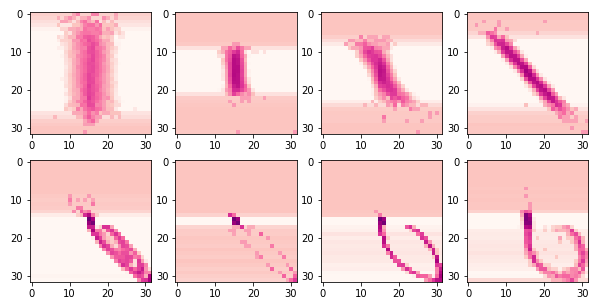
\includegraphics[width=.9\linewidth]{imgs/MTF_LC.png}
\caption{Examples of different types of behavior on MTF of Kepler mission. Only the confirmed objects (exoplanets) are shown here ($32\times 32$ matrix).}
\label{ex:mtf}
\end{figure}
The proposed MTF matrix is useful to illustrate the \textit{global} behavior of all the uneven measurements of light curves in a simpler way, specially if the number of measurements are more than 10 thousand values (as in our case).
The exoplanet transit problem allows us to interpret the light curve transitions channel. For example, the minor state corresponds to the moment when the planet is in front of its host star and blocks the maximum light. While the center state, on positive-negative symmetric matrix, means that the light of the star is measured cleanly (with no eclipsing objects or stellar noise).
 
Figure \ref{ex:mtf} shows different patterns in the transition channel of the MTF images. The objects correspond to confirmed exoplanets light curves of the dataset.
Here, is possible to identify two main types of behavior: diagonal and vertical. Within the diagonal patterns there are two types: ellipse and line, where the latter corresponds to an ellipse with maximum eccentricity ($e=\infty$). 

% + eccentricco + lineal  => lento proceso (periodo alto)
% - eccentrico + ovalado  => rapido proceso (periodo bajo)
The results allow us to discuss the following points.
The diagonal or ellipse patterns are present on those objects whose light curve accounts for clean measurements where eclipses are easily identify. 
Specifically, the level of eccentricity of transitions in MTF is related to the period of the transit object observed on the light curve. 
That is, curves with shorter period (faster transit) show more circular patterns (\textit{smaller eccentricity} on the ellipse) since they have more abrupt transitions between two contiguous points of the time series. 
Instead, a longer period (slower transit) indicates smooth transitions between the states, giving to more diagonal patterns (\textit{high eccentricity}) as observed in Figure \ref{ex:mtf} and Figure \ref{fig:mtf_ex}.
In summary, more eccentricity on the MTF behavior indicates slower orbiting planets.

\begin{figure}[t!]
    \centering
    \subfloat{{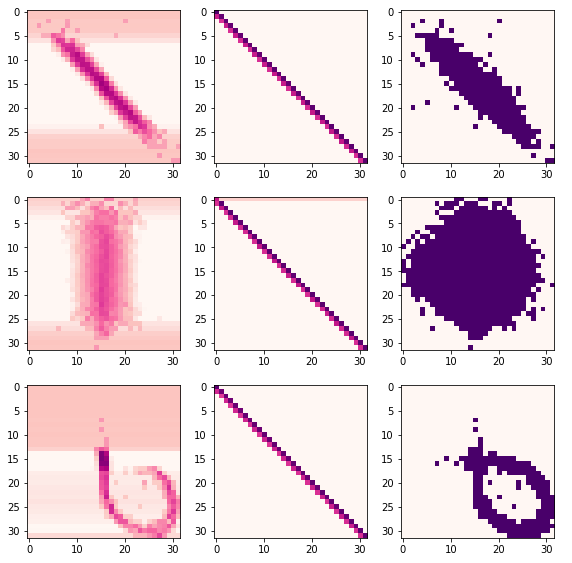
\includegraphics[width=0.45\textwidth]{imgs/Tiny_MTF1.png} }}%
    \qquad
    \subfloat{{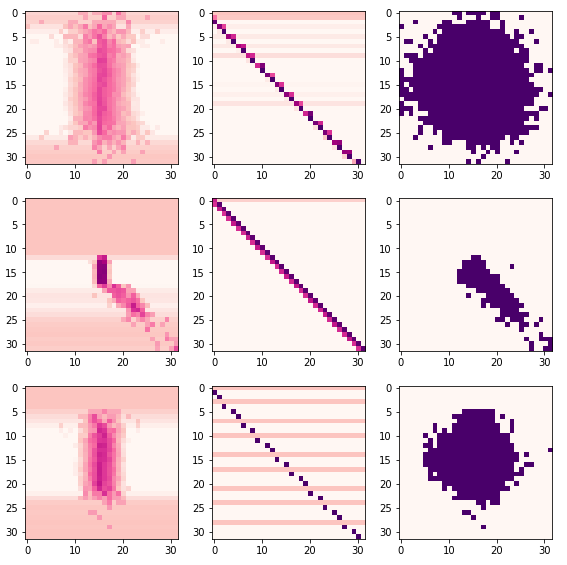
\includegraphics[width=0.45\textwidth]{imgs/Tiny_MTF2.png} }}%
    \caption{Six examples of transition patterns observed on Kepler light curves. In the left is the measurement channel, transitions represented as probabilities (normalized). In the center is the time channel, from the temporal information of the light curve. On the right there is a binarized representation of the measurement channel, 1 if there is a transition between states.}%
    \label{fig:mtf_ex}
\end{figure}
On the other hand, vertical patterns are associated with objects whose light curve presents extremely diffuse transitions. These curves are generally accompanied by a high rate of measurement errors so transitions between states occur \textit{randomly} with the highest concentration at equilibrium states (central zone of the MTF). This phenomenon can be observed in the binary transition images (Figure \ref{fig:mtf_ex}) where there are transitions in almost all the states of the generated MTF. However, when the transitions counts are normalized, vertical patterns are observed.

Note that there are larger behavior patterns that cover the entire range of states. That is, there are measurements near the maximum or minimum value ($1 $ and $- 1$). 
Thus, larger patterns denote a significant number of transitions across the complete spectrum, while shallow patterns denote that the highest concentration of transitions occurs in central states with no focus on extreme values.


\begin{figure}[t!]
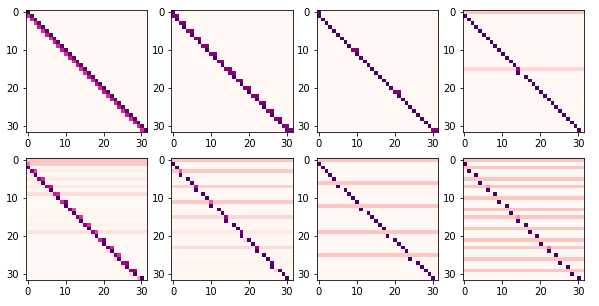
\includegraphics[width=.9\linewidth]{imgs/MTF_Time.png}
\caption{Example of different types of behavior on the time transitions MTF on Kepler mission. Only the confirmed objects (exoplanets) are shown here. $32\times 32$ matrix}
\label{ex:mtf_time}
\end{figure}
Following the analysis for the time channel on the MTF image representation, Figure \ref{ex:mtf_time} shows different observed behavior from confirmed exoplanets on the Kepler mission.
It can be seen that there are some continuous time transitions (exactly diagonal) and others with more discontinuous patterns (diagonal with cuts).
This last one occurs when the light curve transitions have a high delta time that does not meet the specified maximum delta $T_d$, this mean that some sampling rates are greater than the specified by Kepler (half an hour).
The discontinuous patterns are expected because the light curve could have irregularities based on the unevenly-sampled measurements of Kepler dataset, i.e. astronomical phenomenon that obstruct the observation.


\subsection{Model Prediction Analysis}
\begin{figure}[!t]
    \centering
\begin{tabular}{c}
    Confirmed (Exoplanet) predictions (with high confidence) \\
    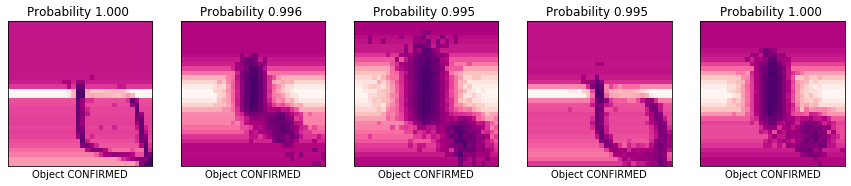
\includegraphics[width=0.95\textwidth]{imgs/MTF_confE_data_v2.png}  \\
    False Positive (Non-Exoplanet) predictions (with high confidence) \\
     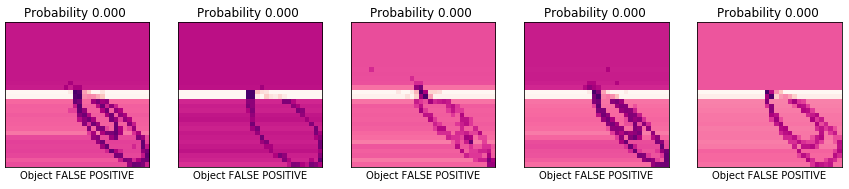
\includegraphics[width=0.95\textwidth]{imgs/MTF_confNE_data_v2.png} \\
    Difficult objects predictions (very low confidence) \\
    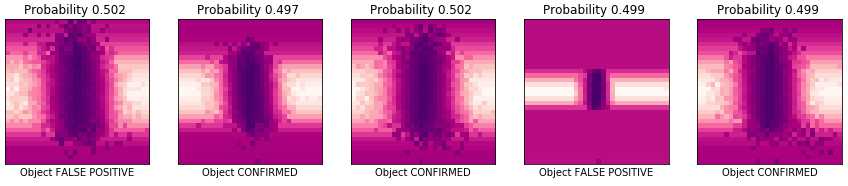
\includegraphics[width=0.95\textwidth]{imgs/MTF_diff_data_v2.png}
\end{tabular}
\caption{Examples on different types of predictions of the KOI objects (MTF).}
\label{fig:mtf_pred_ex}
\end{figure} %cmap es RdPu, sin limite en lognorm (el valor maximo y mas oscuro, no es 1)
Figure \ref{fig:mtf_pred_ex} shows examples of our representation for the KOI objects (MTF) that the 2D CNN model predicts with high reliability. We use the model probability predictions, $p(y=\texttt{confirmed})$, to understand the shape of objects with probability close to 1 (most likely confirmed) and close to 0 (most likely false positive). 

As previously stated, the standard well defined transits (without noise or random behavior) are objects with bottom right ellipse patterns, where the objects predicted as confirmed have more thick pattern than the objects predicted as false positives.
There also seems to be a second ellipse on the false positive objects, meaning perhaps a binary system (two stars eclipsing each other with two statistical different transits). 
These two intrinsic characteristic could be the factors that our model consider in order to classify as a certain class: analyze the type of pattern into the bottom diagonal (\textit{it is clearly only one ellipse?}) and how thick are the patterns.

In addition, we show the most difficult objects to classify, where the model is not sure of the class label (probability close to 0.5).
On this case it can be seen a big spot on the center with no clear inclination to the bottom right. These patterns are the vertical ones commented earlier which we associate to random transitions. 
This clarifies the difficulties of classify these types of objects despite the fact that some of them have an orbiting exoplanet. Therefore, there does not appear to be a clear difference between objects with or without exoplanets.

\section{Conclusion}

We propose an image representation based on Markov Transition Fields for unevenly-sampled light curves than can be combined with deep learning models. 
We apply this technique to the exoplanet detection problem, harnessing the power of 2D convolutional neural network as simpler alternative to deep learning methods than processing the raw representation of light curves.

The results over the KOI dataset of the Kepler mission takes around 20 minutes to process. Also, our method is faster to execute and lighter in terms of memory consumption, yet it offers a competitive performance of 77.01\% in the \textit{F1-score} (macro averaged) with respect to similar techniques. 

%We also show that the proposed method could be more effective for the learning task.

%The main advantage of our proposal is the execution time. This will help experts to generate early predictions of exoplanets, without the need to wait days or hours for another algorithm to generate a similar prediction.

Based on the visual interpretation of the MTF images content (global transition behavior), we plan to inspect in detail the least and most likely semi-continuous transitions in order to produce new knowledge from the specific local patterns of the time series. In addition, we have the intention to improve the sparse matrix representation investigating the use of kernel-based estimation in the continuous space.





\section*{Acknowledgments}
This research was possible due to the funding of \textit{Programa de Iniciaci\'on Cient\'ifica} PIIC-DGIP of Universidad T\'ecnica Feder\'ico Santa Mar\'ia, ANID-Basal Project FB0008 (AC3E) and ANID PIA/APOYO AFB180002 (CCTVal).

\bibliography{mybibfile}

\end{document}